\documentclass[12pt]{article}
\usepackage[T1]{fontenc}
\usepackage[slovak]{babel}
\usepackage{mathptmx}

\usepackage{caption}
\usepackage{subcaption}

\usepackage[width=\textwidth]{svg}

\usepackage[a4paper,left=35mm,
                    right=25mm,
                    top=25mm,
                    bottom=25mm]{geometry}

\linespread{1.5}   % 1.5 riadkovanie

\AddToHook{cmd/section/before}{\clearpage}

\def\nazovprace{Botanica - simulátor rastlín na báze celulárnych automatov}
\def\autori{František Knapec, Michael Sklenka, Marek Beňo}

\begin{document}

\begin{titlepage}
	\setlength{\parindent}{0pt}

	\begin{center}
		Gymnázium \\
		Veľká okružná 22, 010 01 Žilina

		\vspace{7cm}
		\Huge \nazovprace

		\vspace{1.13cm}
		\Large Stredoškolská odborná činnosť

		\vspace{2.12cm}
		\normalsize Č. odboru: 11
	\end{center}

	\vfill

	\begin{minipage}{0.75\textwidth}
		Riešitelia: \autori \par
		Ročník štúdia: 4.
	\end{minipage}
	\hfill
	\begin{minipage}{0.23\textwidth}
		\hfil % basically align right
		\begin{tabular}{rc}
			Mesto: & Žilina \\
			Rok:   & 2025
		\end{tabular}
	\end{minipage}
\end{titlepage}

\begin{titlepage}
	\setlength{\parindent}{0pt}

	\begin{center}
		Gymnázium \\
		Veľká okružná 22, 010 01 Žilina

		\vspace{7cm}
		\Huge \nazovprace

		\vspace{1.13cm}
		\Large Stredoškolská odborná činnosť

		\vspace{2.12cm}
		\normalsize Č. odboru: 11
	\end{center}

	\vfill

	\begin{minipage}{0.75\textwidth}
		Riešitelia: \autori \par
		Ročník štúdia: 4. \par
		Školiteľ: PaedDr. Jana Pekárová, PhD.\par
		Konzultant: Ing. Tomáš Milet, PhD.
	\end{minipage}
	\hfill
	\begin{minipage}{0.23\textwidth}
		\hfil % basically align right
		\begin{tabular}{rc}
			\\ \\
			Mesto: & Žilina \\
			Rok:   & 2025
		\end{tabular}
	\end{minipage}
\end{titlepage}

% zapocitaj strany
\setcounter{page}{3}

%
% Čestné vyhlásenie
%

\thispagestyle{empty}

\noindent
\textbf{Čestné vyhlásenie:}

\noindent
Prehlasujeme, že sme prácu na tému
\nazovprace \space
vypracovali samostatne s~použitím literatúry uvedenej v~zozname použitej literatúry.
Zároveň prehlasujeme, že sme predloženú písomnú prácu neprihlásili a ani neprezentovali
v žiadnej inej súťaži, ktorá je pod gestorstvom MŠMVVaŠ SR. Sme si vedomí zákonných dôsledkov,
ak v~nej uvedené údaje nie sú pravdivé.

\newpage


%
% Poďakovanie (nepovinné)
% TODO: chceme?
%

% \thispagestyle{empty}
% 
% \null
% \vfill
% 
% \noindent
% \textbf{Poďakovanie}
% 
% \noindent
% Toto je poďakovanie
% 
% \vspace{8cm}
% \newpage


%
% [x] Obsah
% [ ] Zoznam skratiek, značiek a symbolov (nepovinné)
% [ ] Zoznam tabuliek, grafov a ilustrácií (nepovinné)
%

\thispagestyle{empty}
\tableofcontents

%
% The work :)
%

\addcontentsline{toc}{section}{Úvod}
\section*{Úvod}

\section{Problematika a prehľad literatúry}

Táto práca sa zaoberá implementovaním rastlín do digitálnej podoby a následným
simulovaním ich správania relatívne k podmienkam, v ktorých sa nachádzajú,
ako aj k iným rastlinám v ich okolí. Do tejto práce patrí aj vyobrazenie
rastlín v trojdimenzionálnom priestore. Pôjde aj o schopnosť dlhodobého
pozorovania ekosystému naprieč časom.

Ľudia k problému tvorenia digitálnych rastlín postupovali rôznymi spôsobmi,
avšak väčšina z nich len realistické rastliny vykresľovali, ako je napríklad
známy príklad L-systémov,\footnote{
	Lindenmayerov systém - https://en.wikipedia.org/wiki/L-system
	}
ktorý je založený na opisovaní štruktúry rastlín
sériou pravidiel, ako je napr. otočenie, vytvorenie úsečky alebo
vrátenie sa na určitú pozíciu. Ďalej sa štruktúra zdokonaľuje za pomoci
algoritmu, ktorý nahrádza časti jej série pravidiel za iné, dopredu určené
a detailnejšie série. Tento postup dokáže vytvoriť celkom realistické rastliny
ako je znázornené na obr. \ref{obr:priklad l-systemu}.

\begin{figure}[ht]
	\centering
	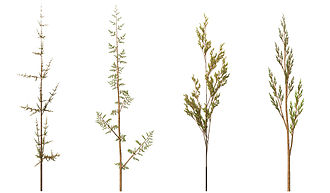
\includegraphics[width=0.5\textwidth]{res/Fractal_weeds.png}
	\caption{Príklad trávy vygenerovanej s použitím L-systému v 3D}

	\footnotesize (zdroj: https://en.wikipedia.org/wiki/L-system)

	\label{obr:priklad l-systemu}
\end{figure}

Toto riešenie a jemu podobné avšak dané rastliny len
vytvárajú, ale našim cieľom je ich aj simulovať. Na samotnú simuláciu
s vytvorilo viacero algoritmov s vlastnými pozitívami, ale aj zápormi.


\subsection{Spôsoby simulovania rastlín}

TODO: write

\subsubsection{Fyzikálne založené modelovanie}

Jedná sa o simuláciu využívajúcu bodoy, ktoré sú navzájom prepojené pružnými
štruktúrami, na ktoré konajú rôzne sily, ako je gravitácia, vietor
a napätie. Tento štýl simulovania je populárny najmä vo filmoch a fyzikálnych
simuláciách, ako názov napovedá, no neposkytuje vytváranie týchto štruktúr,
ktoré musia byť napred vytvorené. Tým pádom nemôžeme pozorovať dlhodobý
vývin ekosystému.
% TODO: ukážky, citácie, zdroj
% Tu by sa hodili nejaké ukážky kódu alebo hotových rastlín,
% tiež citácie z literatúry.

\subsubsection{Simulácia pomocou strojového učenia}

% TODO: fixni

Strojové učenie\footnote{
	Strojové učenie - https://en.wikipedia.org/wiki/Machine\_learning
	}
je obrovský nástroj, čo sa týka nielen simulovania rastlín.
Je všestranný a dokáže si poradiť s rôznymi zadaniami, od simulácie
založenej na chemických procesoch, vonkajších činiteľoch alebo
procesovo založenom skúmaní a pod.
% Čo je procesovo založené skúmanie? Všetky pojmy treba dobre popísať, vysvetliť...
Práca
	% Aká práca? Tá vaša? Toto by som sem ešte neplietla... skôr popíšte,
	% ako funguje strojové
sa môže teoreticky považovať za strojové
učenie, keďže fungujú na rovnakom princípe: máte niekoľko agentov, ktorý
zo začiatku konajú náhodné akcie a tí, ktorí boli najefektívnejší,
posielajú svoj kód ďalej, pre ďalšie generácie a z tých sa znova zoberú
tí najlepší atď.
Rozdiely % Rozdiely voči čomu???
sú v tom, že agenti v strojovom učení majú
neurálne štruktúry, ktoré im hovoria čo a ako. Rastliny v tomto projekte
tieto štruktúry neobsahujú, ale namiesto toho majú svoj genetický kód,
ktorý pracuje na podobnom princípe.
Taktiež % Tiež do inej časti... Tu sa spomína Botanica, no ešte ani nebolo
		% uvedené, čo to je. Pozor na súslednosť textov.
strojové učenie má dopredu
určený počet agentov, ktorý môžu testom prejsť. Botanica funguje na
princípe „survival of the good-enough“ alebo „prežitie dostatočných“.

\subsubsection{Celulárne automaty}

Celulárne automaty\footnote{
	Celulárne automaty - https://en.wikipedia.org/wiki/Cellular\_automaton
	}
je názov pre matematický model a nástroj pre
simuláciu. Jedná sa o starší koncept, ktorý obsahuje štvorcovú sieť
so „zafarbenými“ políčkami. Každá farba je určitý stav, ktorý má špecifické
správanie závisiace od okolitých políčok.

% TODO: obkec, že sme vybrali CA a prečo

\newpage %? move to a different part?
\subsection{Celulárne automaty}

CA môžeme charakterizovať štyrmi základnými pojmami: mriežka (štorcová sieť),
stavy buniek, pravidlá a diskrétne časové zmeny.
Tieto pojmy z CA robia záležitosť, ktorá je diskrétna ako v čase, tak aj v
priestore a umožňuje nám dôkladné pozorovanie. % TODO: rewrite this sentence

Mriežka môže byť v rôznych prípadoch jednorozmerná, dvojrozmerná alebo ako je
to v našom prípade aj trojrozmerná,
%? maybe remove the bottom one?
avšak najčastejšie využívanou mriežkou je
dvojrozmerná mriežka pozostávajúca zo štvorcových buniek.

Každá bunka v mriežke nadobúda jeden z viacerých stavov ako napríklad „živá“
alebo „mŕtva“ v najjednoduchšom systéme, teda binárnom.

Pravidlá definujú správanie bunky v závislosti jej stavu od susedov. Susedov
môžeme taktiež definovať 2 spôsobmi v N+1 dimenziách, ak nerátame diagonálne
bunky ako susedné, ide o von Neumannove susedstvo, ak rátame aj diagonály,
ide o Moorove susedstvo. % Citácia z literatúry???

Zmena času sa odohráva v diskrétnych časových odsekoch, toto má za príčinu
našu schopnosť sledovať zmeny všetkých stavov buniek naraz.

\subsubsection{Príklady na klasické CA}

Conwayova hra života je pravdepodobne najznámejší príklad celulárnych
automatov. Jedná sa o dvojrozmernú štvorcovú mriežku, kde bunky majú dva stavy:
„živé“ alebo „mŕtve“, ich stav závisí od stavu okolitých buniek.

Wolframove celulárne automaty kategorizujú správanie jednorozmerných CA.
Sú schopné generovať komplexné a nepredpokladateľné vzorce, ak k ním pridáme
druhú dimenziu reprezentujúcu čas z nekomplexných pravidiel.

Viacrozmerné CA využívajú tri alebo viac dimenzií a sú prevažne využívané
na modelovanie fyzikálnych javov, ako je tvorba kryštalických štruktúr
alebo difúzia. % Citácia, ukážte nejaké príklady...

\subsubsection{Príklady CA zamerané na simuláciu rastlín}

„Simulation of root forms using cellular automata model“ - zameriava sa na
korene rastlín a dopad premenných ako napr. živiny v pôde, voda a prekážky
v raste. Jedná sa o prácu, ktorá je viac zameraná na matematický rast koreňov,
avšak my sme rast koreňov simulovali genetikou.
% Trošku to rozveďte. Pri návrhu vlastného systému generovania rastlín sme
% sa inšpirovali rôznymi jestvujúcimi softvérovými riešeniami. Na korene
% rastlín a dopad rôznych faktorov sa zameriava...

„A Model Based on Cellular Automata for the Simulation of the Dynamics of
Plant Populations“ - zameriava sa na 2D simuláciu heterogénnej populácie
rastlín, zameraná na konkurenciu medzi druhmi, rýchlosť rastu a interakcie
s prostredím.

\section{Ciele práce}

Cieľom tejto práce je vytvorenie aplikácie schopnej vytvárania a simulácie
pseudo-rea\-listických rastlín v trojrozmernej mriežke pomocou celulárnych
automatov a implementovanej genetiky.
Tieto rastliny by mali byť schopné reagovať na prostredie v reálnom čase
a adaptujú svoje správanie, tvar a iné charakteristiky v závislosti
od podmienok, v ktorých sa nachádzajú.

Veríme, že tieto metódy sú využiteľné ako na vytváranie dynamického
a nerepetetivného prostredia vo video-hrách, tak aj na viac vedecké účely
ako pozorovanie správania rastlín vo virtuálne vytvorených podmienkach
a ich ideálne charakteristiky za daných podmienok.
% TODO:
% Toto je výborne sformulované. Chcelo by to ešte rozmeniť na drobné.
% Napr. takto Výstupom našej práce bude softvérové prostredie Botanica,
% ktoré bude mať tieto vlastnosti: 1), …

\section{Materiál a metodika}

Simulátor % Toto je zase tak uprostred práce.
		  % Treba popísať vývoj krok za krokom. Cieľom našej práce bola tvorba
		  % prostredia Botanica. Jej vývoj zahŕňa kombináciu rôlznych
		  % technológií: samotný simulátor bol...
bol vytvorený vo Visual studio code za pomoci jazykov C++ a GLSL.
Ďalej sme využili knižnicu GLFW, ktorá pomáha s vývojom aplikácií vďaka tomu,
že poskytuje jednoduché API na vývoj aplikácií. Ďalej sme využili Glad,
softvér, ktorý generuje multi-jazykové loadery, matematickú knižnicu GLM
a logovaciu knižnicu spdlog. Na vykreslenie trojrozmerného prostredia sme
využili OpenGL.
% Tu by sa ešte hodilo niečo ako fázy práce, koľko čo trvalo
% alebo ako ste si to rozdelili...

%? Nova cast
\section{Aplikácia}

Na realizovanie algoritmu sme vyvinuli jednoduchú aplikáciu, ktorá má všetky
potrebné Na realizovanie algoritmu sme vyvinuli jednoduchú aplikáciu, ktorá má
všetky potrebné prostriedky na demonštráciu všetkých aspektov tohto algoritmu.
Aplikácia umožňuje vizualizáciu rastu rastlín na základe celuárnych automatov
a poskytuje možnosť meniť parametre simulácie na dosiahnutie idealného vzhľadu
rastlín.

\subsection{Svet}

Svet aplikácie pozostáva z mriežky buniek o rozmeroch 32x32x32 voxelov.
Každý voxel nadobúda určitý stav. Môže sa jednať o časti rastlín (stonka, list,
koreň alebo ovocie), ale aj o časti terénu (vzduch, voda, pôda).

\subsubsection{Perlinov šum}

Terén na určenie svojej výšky, aby nebol len rovina, využíva funkciu zvanú
Perlin noise. Perlin noise, je spôsob generovania hodnôt, ktoré sú náhodné,
pričom body, ktoré sú si susedné, sa v hodnotách moc nemenia. Toto vytvára
hodnoty, ktoré sa dajú skvelo využiť na generovanie realistického terénu.
Čo sa týka algoritmu na jeho generovanie, v určitých miestach sa vytvoria
vektory s náhodným smerom (modrý). Z bodov (červené), ku ktorým chceme pripísať
hodnoty, sa vytvoria vektory smerujúce k týmto miestam (zelené). Z náhodného
vektoru a vektoru smerujúceho z bodu sa vytvorí skalárny súčin a tým dosiahneme
hodotu v danom bode.

Avšak väčšinu času sa hodnoty nepočítajú len pre jeden náhodný vektor,
ale viacero, najčastejšie 4 najbližšie a hodnoty ich skalárnych súčtov
sa spriemerujú. Často sa využíva aj viacero oktáv, pričom každá oktáva generuje
viacej náhodných vektorov, ktoré ovplyvňujú menej buniek, ako predchádzajúca
oktáva, avšak vplýva menej na výslednú hodnotu. Ak vyjadríme hodnoty bodov
farebnou škálou kde vyššie hodnoty sú viac biele a nižšie viac čierne dostaneme
nasledujúci obrázok:

\begin{figure}[h]
	\centering

	\begin{subfigure}[t]{0.49\textwidth}
		\centering
		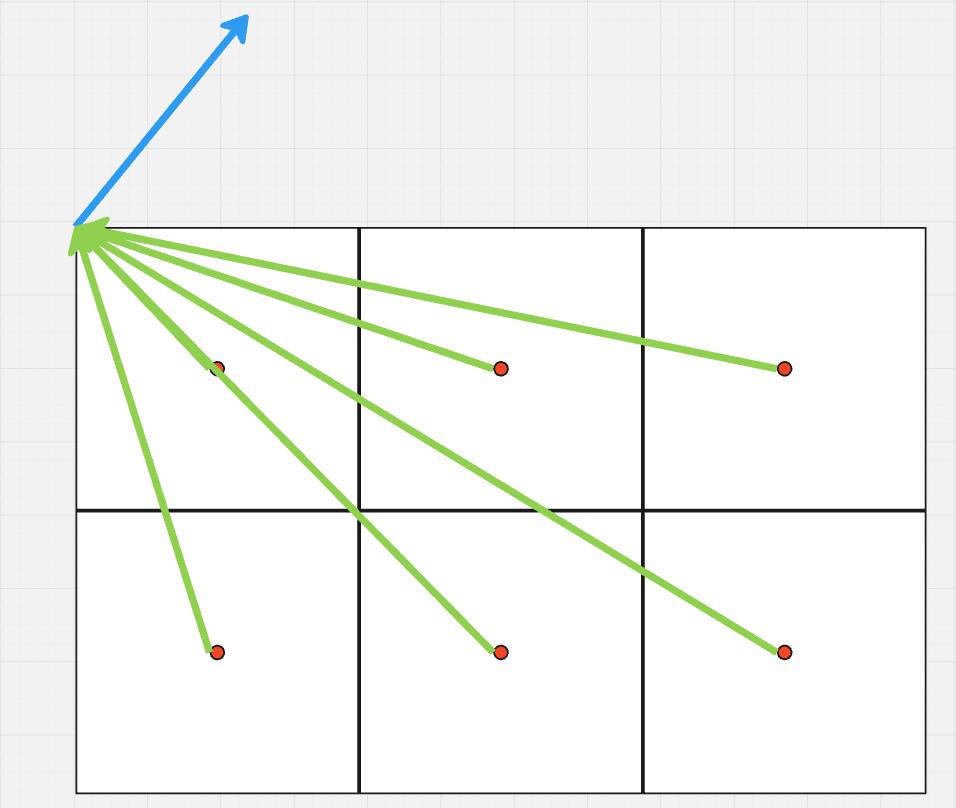
\includegraphics[width=0.7\textwidth]{res/prelinov_sum.png}
		\caption{...}
		\label{obr:perlinov sum}
	\end{subfigure}
	\hfill
	\begin{subfigure}[t]{0.49\textwidth}
		\centering
		
\includegraphics[width=0.6\textwidth]{res/perlinov_sum_textura.png}
		\caption{...}
		\footnotesize (zdroj: https://en.wikipedia.org/wiki/Perlin\_noise)
		\label{obr:perlinov sum textura}
	\end{subfigure}

	\caption{Perlinov šum}
\end{figure}

Naša aplikácia, vďaka jej obmedzenej veľkosti, využíva 4 vektory umiestnené
na rohoch simulácie a iba 1 oktávu.

\subsubsection{Vytváranie terénu}

Vytváranie sa začne vytvorením Perlin noisu, poďla ktorého sa určí jeho výška.
Pre každú dvojicu súradníc X a Z sa vytvorí hodnota Perlin noisu. Táto hodnota
bude ovplyvňovať os Y. Každý voxel, ktorého hodnota súradnice Y je nižšia alebo
rovná hodnote noisu v X,Z bude voxel terénu. Inak sa bude jednať o voxel
vzduchu. Na vytvorenie voxelov vody sa nastaví hodnota, ktorá bude označovať
hladinu vody a ak hocaký voxel vzduchu má hodnotu Y menšiu alebo rovnú ako táto
hodnota, zmení sa na vodu. Táto hodnota nie je spojená s noisom, ide o jedno
číslo univerzálne pre celú simuláciu. Zoberme si príklad: máme zmenšenú
simuláciu a pre každú dvoju X,Z pripadajú len 4 voxely [0,1,2,3]. Tieto voxely
majú rovnaké súradnice X,Z ale odlišné Y, ktorá korešponduje s ich číslom.
Vytvoríme Perlin noise, ktorý bude mať pre danú dvoju X,Z hodnotu 1. To
znamená, že voxely s hodnotou Y 0 a 1 sa premenia na voxely pôdy a voxely 2,3
na voxely vzduchu. Ďalej hladina vody má hodnotu 2, takže voxel 2, ktorý bol
pred tým vzduch sa premení na vodu.

\subsubsection{Živiny}

Simulácia obsahuje rôzne živiny, vodu a vzduch, tieto veci rastlina potrebuje
získavať aby rástla a prežila. Voda a vzduch majú zastúpenie v podobe ich
voxelov. Pôda obsahuje vodu a živiny. Každá živina napomáha rôznym procesom
rastliny, ako napríklad fotosyntézovať, čerpať vodu alebo získavať viac živín.
Ich nadbytok má kladný vplyv na rastliny, avšak ich nedostatok má zase
negatívny. Toto pridáva na komplexnosti, realizme a dovoľuje nám získať rôzne
typy rastlín, podľa toho, ku ktorým živinám majú alebo nemajú prístup.
Napríklad ak rastlina nemá dostatok dusíka, ktorý je v simulátore dôležitý
na fotosyntézu, rastlina to musí kompenzovať viacerými listami, inak zanikne.
Živiny sú 3, dusík, draslík a fosfor, pričom bola snaha o to, aby napomáhali
realistickým precesom, ktoré tieto prvky vyžadujú. Draslík je nápomocný pri
absorpcii vody, takže ak má rastlina nadbytok draslíka, efektívnejšie získava
vodu. Využitie dusíka je široké, ale v simulátore je jeho funkcia obmedzená
len na zlepšenie fotosyntézy, keďže je hlavnou zložkou chlorofylu. Fosfor je
rovnako ako dusík dôležitý v rôznych častiach, avšak v simulátore je zameraný
na absorpciu živín.

\subsection{Rastliny}

Rastliny sú v tomto simulátore objekty so spoločnou „triedou.“ Trieda je
predloha premenných a špeciálnych funkcií zvaných metód, ktoré využívajú
jednotlivé entity, taktiež známe ako objekty. Takáto šablóna nám umožňuje
jednoducho a usporiadane vytvárať rastliny, pretože nemusíme písať samostatný
kód pre každú rastlinu.

\subsubsection{Premenné v rastlinách}

Rastliny majú viacero premenných. Ich hlavnou úlohou je opísať stav rastliny.
Medzi ne paria údaje o skonzumovaných živinách za toto kolo, zoznam všetkých
voxelov, v ktorých sa nachádzajú časti rastliny a ich gény. V premenných
taktiež máme aj bonusy pre živiny. Hovoria nám o nadbytku alebo nedostatku
živín. Čo tieto bonusy robia je rozbrané v kapitole „Živiny“.

\subsubsection{Rastlinné voxely}

Fyzické zobrazenie rastlín sa skladá zo špecializovaných voxelov, ktoré
v mriežke reprezentujú ich časti. Tieto voxely taktiež voláme aj bunky.
Existujú 4: bunky koreňov, stonky, listov a ovocia. Každá skupina buniek plní
vlastnú úlohu. Koreň má za úlohu rastline získať živiny a vodu, to dosahuje
odoberaním týchto živín z okolitých voxelov. Koreň môže vzniknúť iba na
miestach, kde je pôda. Úlohou listu je fotosyntéza, tú dosiahne tým, že
skontroluje, či políčka nad ním sú vzduch. Predpokladáme, že na voxeli vzduchu
priamo svieti slnko. Môže nahradiť políčka kde je vzduch. Stonka uskladňuje
živiny pre rastlinu.  Rastie iba zvislo. Ovocie vytvára nové rastliny
s rovnakým genetickým kódom ktorý trochu zmutuje. Na pár kôl nahrádza 1 list,
ktorý sa po premenení ovocia na novú rastliny znova zmení na list.

\subsubsection{Genetika}

Na základe genetiky rastliny rozhodujú, aké časti majú rásť (listy, stonka…)
a v prípade listov a koreňov sú gény, ktoré hovoria, akým smerom majú rásť.
Takže existujú 3 gény: čo má rásť, kde majú rásť korene a kde majú rásť listy.
Gén „čo má rásť“ je vo všetkých prípadoch list so 4 číslami. Sú 4, pretože sú 4
typy buniek, ktoré môže rastlina rásť: korene, listy, stonku a ovocie. Čísla
v týchto listoch označujú, ako moc chce daná rastlina danú časť rásť. Takže
ak má rastlina v časti označujúcu stonku 2 a koreň 10, daná rastlina bude
chcieť koreň rásť 5-krát viac, ako stonku. Ktorú časť bude rastlina naozaj
rásť sa rozhoduje náhodne. Takže ak sa vrátime k nášmu príkladu dokopy 2+10=12,
takže to je ako keby naša rastlina hádzala s 12-stenou kockou. Ak padne číslo,
ktoré je väčšie ako 2, rastie koreň, inak stonka. Gény „kde majú rásť korene“
a „kde majú rásť listy“ sú rovnaké, len ako ich názov hovorí, jeden sa zaoberá
koreňmi a druhý listami. Sú to listy s 26 číslami. Je ich 26 pretože bunka má
v trojrozmernom priestore 26 susedov, ak rátame aj diagonály. Zvyšok funguje
rovnako ako gén „čo má rásť“. Takže sú tam čísla, ktoré označujú
pravdepodobnosť rastu do toho smeru. Ak sa tieto 2 gény zavolajú vyberie
sa náhodná bunka (list alebo koreň, podla toho, ktorý gén sa zavolá) a ak
nemôže rásť do toho smeru, tak sa vyberie iná bunka, ak žiadna nemôže rásť,
vyberie sa iný smer.

\subsection{Algoritmus}

Ako bolo spomínané, simulácie nebeží súvisle, ale v časových „krokoch“.
Za každý krok sa vykonajú určité akcie, tzv. cyklus. Tieto akcie slúžia na beh
simulácie a starajú sa o veci ako je rast rastlín, ich vzniknutie, smrť atď.
Algoritmus za týmto môžeme rozdeliť do nasledujúcich častí, ktoré sú spísané
chronologicky, čiže postupne, ako ich simulácia vykonáva.

\subsubsection{Vznik rastlín}

Je jediná časť algoritmu, ktorá nebeží v krokoch, ale iba raz, a to na začiatku
simulácie. Po vytvorení terénu sa vyberie náhodné miesto na jeho povrchu, kde
je pôda, a tam vznikne rastlina. Toto sa dá opakovať viackrát, na vytvorenie
viacerých rastlín. Takéto rastliny sa skladajú z 1 koreňa, 1 stonky a 1 listu.
Ich genetika je náhodná, keďže ju nemôžu dediť z materínskych rastlín, ktoré
neexistujú.

\subsubsection{Redistribúcia živín}

Je prvá akcia, ktorá sa vykonáva v cykle, každý krok simulácie. Živiny sú totiž
ukladané v dvoch listoch, jeden permanentný, ktorý drží informácie o počte
živín a vody zo začiatku simulácie a druhý dočasný, z ktorého rastliny čerpajú.
V tomto bode sú odobrané všetky živiny, ktoré sa udržiavajú v rastlinách a list
dočasných živín je znovunastavený na hodnoty rovné permanentnému listu.
Toto umožňuje rastlinám znovu brať živiny v novom cykle.

\subsubsection{Zasadenie rastlín}

Ak má rastlina ovocie, ktoré existuje po určitú dobu, tak sa z neho stane nová
rastlina. Rozdiel vo vzniku a zasadení je, že tentokrát genetický kód nie je
vygenerovaný náhodne, ale ho rastlina zdedí zo svojej materinskej rastliny,
pričom v každej časti genetiky jednu hodnotu náhodne zmení, teda „zmutuje“.

\subsubsection{Produkcia}

V tejto fázy rastlina získava živiny vďaka svojím bunkám, konkrétne listom
a koreňom. Listy sa pozrú na bunky horizontálne nad nimi a podla toho, koľko
z nich sú vzduch, „produkujú“ svetlo. Korene zase pozrú bunky v ich susedstve
a podla toho generujú živiny a vodu. Koľko z okolitých buniek dokážu listy
a korene dostať je určený samozrejme, počtom živín v bunkách terénu, z ktorého
rastlina čerpá, ale rastlina nezoberie jednoducho všetky živiny v okolitom
teréne. Maximálny počet živín, ktoré dokáže bunka získať je stanovený
konštantou a jej bonusom zo živín. V stonkách sa uskladňujú živiny, čiže
rastlina nemôže skonzumovať viac, ako jej to limit odvodený z počtu buniek
stoniek dovoľuje. Na príklad: chceme fosfor, je koreň s 5 okolitými bunkami,
pričom každá obsahuje 15 jednotiek fosforu. Konštantu produkcie máme 10,
povedzme že máme bonus pre fosfor krát 1.2, čiže z každej dokážeme brať až 12
jednotiek. To máme do kopy 60 jednotiek, ktoré dokáže daný koreň získať,
ale povedzme, že kapacita stoniek je len 50, takže náš koreň nakoniec
vyprodukuje len 50 jednotiek fosforu.

\subsubsection{Smrť}

Ak rastlina má nedostatok jednej zo živín, zomrie. Koľko živín rastlina
potrebuje na prežitie je odvodené od jej veľkosti, čiže počtu jej voxelov
a premennej určenej na začiatku simulácie zvanej „obtiažnosť“. Ako príklad
dajme rastlinu s 10 bunkami, obtiažnosťou 5 a 45 jednotkami živiny, ktorú
pozorujeme ako napr. fosfor. Vynásobíme počet buniek a obtiažnosť, takže
10*5=50. To znamená, že rastlina potrebuje najmenej 50 jednotiek zo všetkých
živín, aby prežila. Keďže má len 45 jednotiek fosforu, zomrie na jeho
nedostatok.

\subsubsection{Kalkulácia bonusov zo živín}

Podobne ako smrť, sa odvíja od veľkosti rastliny a konštanty. Pre každý bonus
sa ráta zvlášť a keďže tento krok je až na konci cyklu v úplne prvom cykle
simulácie majú všetky rastliny bonusy rovné 1.

\section{Výsledky práce}
\section{Diskusia}
\section{Závery práce}
\section{Zhrnutie}
\section{Zoznam použitej literatúry}
% Prílohy (nepovinné)

\end{document}